\subsection{Schema-Modell}
\label{sec:schema_model}

\begin{figure}[t]
    \centering
    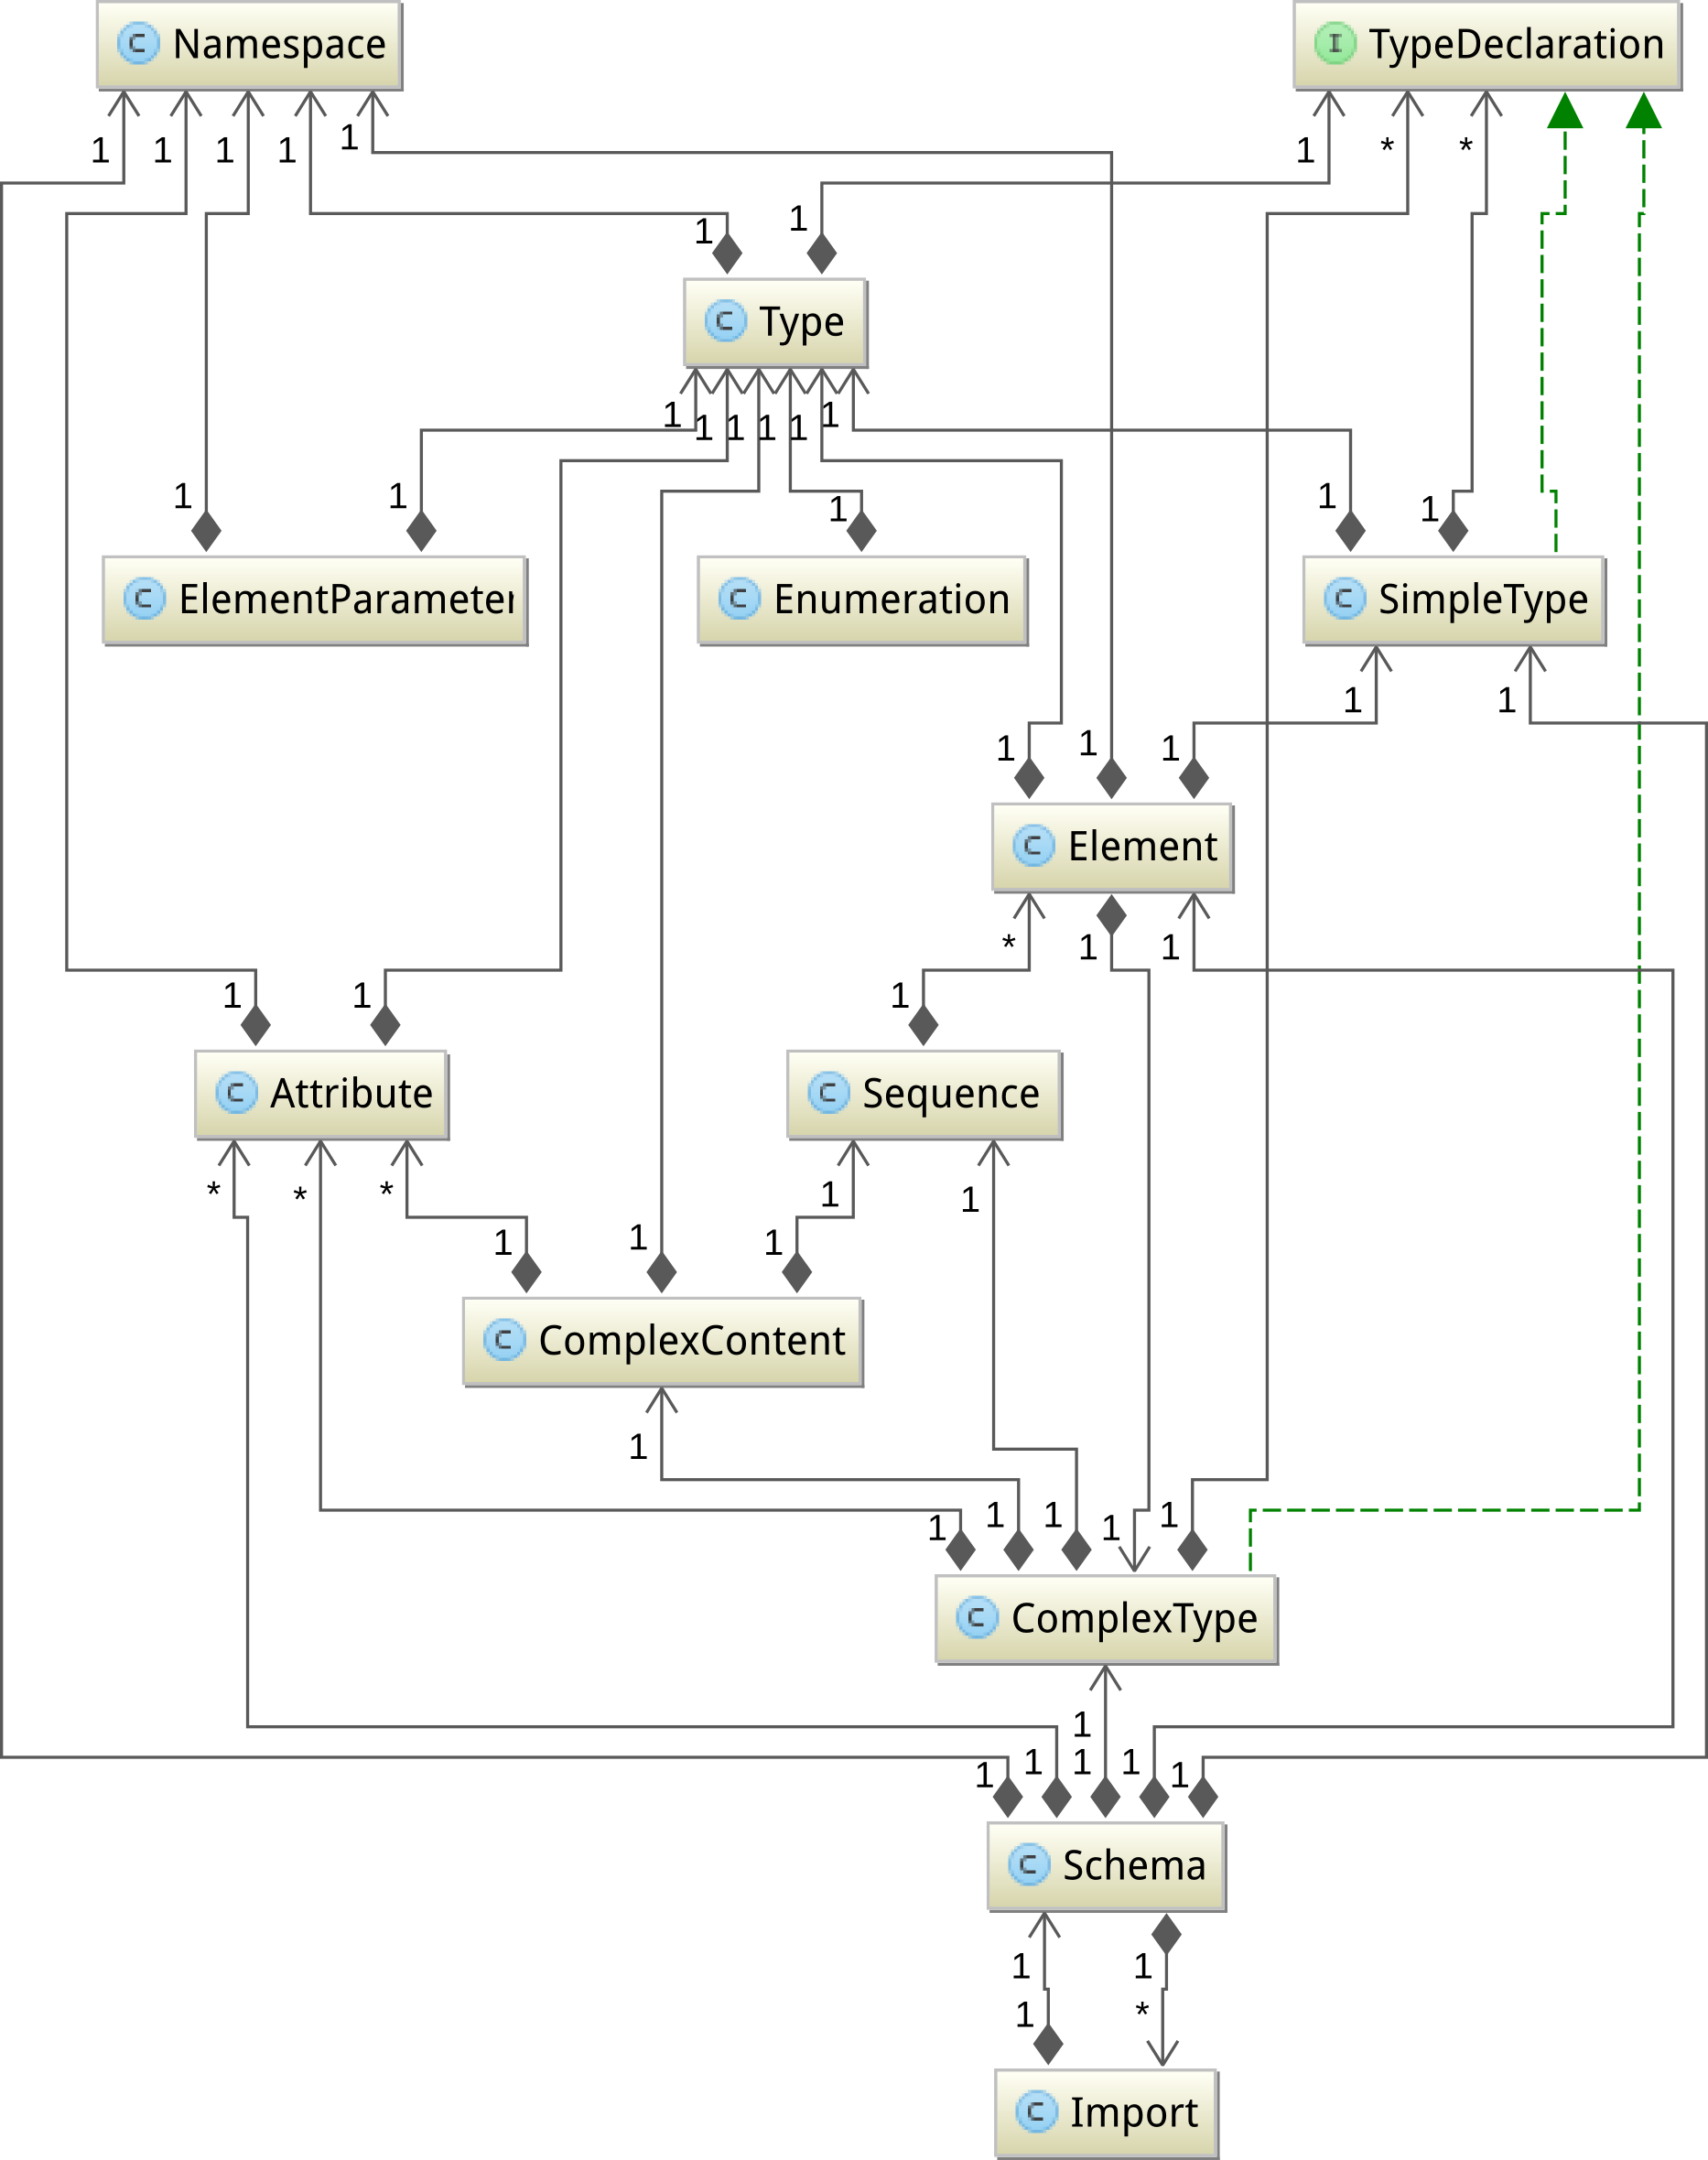
\includegraphics[width=0.6\textwidth]{resources/typemodel}
    \caption{\textsc{Uml} Klassendiagramm des Schemadatenmodells}
    \label{fig:schema_model}
\end{figure}

Wurzel des Schemadatenmodells ist die Klasse \textbf{Schema}. Ein Schema kann Objekte vom Typ \emph{Complex-} und \emph{SimpleType} sowie \emph{Attribute} und \emph{Element} enthalten.

\textsc{Xsd}-Dateien (siehe \cref{sec:xsd}) erlauben das importieren anderer Schemadefinitionen, die Klasse \textbf{Import} ermöglicht dies im Schemamodell. Sie besitzt ein Objekt des zu importierenden Schemas sowie eine \gls{URI} auf die zugehörige \textsc{Xsd}-Datei.

Primitive Schematypen werden durch die Klasse \emph{SimpleType} abgebildet. Objekte dieser Klasse enthalten eine Kennzeichnung der Art des SimpleType (Enumerator, Liste, einfacher Wert) und bei Enumeratoren zusätzlich die einzelnen Enumeratorwerte, sowie die Angabe des Basisdatentyps.

Die \textbf{ComplexType}-Klasse repräsentiert die gleichnamigen strukturierten Typen aus der Schemabeschreibung. 
Ein ComplexType kann Attribute, Elemente, Elementsequenzen und strukturierten Inhalt (\emph{ComplexContent}) enthalten.

\textbf{ComplexContent} kann die gleichen Objekte wie \emph{ComplexType} enthalten, sowie einen Basistyp der Erweitert oder Eingeschränkt wird (\enquote{derivation by extension/restriction}).

Attribute werden durch die gleichnamige Klasse \textbf{Attribute} gekapselt, sie besitzen einen Attributnamen sowie eine Definition ihres Typs.

Elementsequenzen werden durch die \textbf{Sequence}-Klasse repräsentiert. Sie enthält einen Reihenfolgeindikator (siehe \cref{sec:xsd}) und die Elemente der Sequenz.

Objekte der Klasse \textbf{Element} besitzen einen Bezeichner, sowie einen Complex- oder SimpleType und optional eine Angabe der Auftrittshäufigkeit. Die Klasse \emph{ElementParameter} dient nur zur Kapselung der Daten welche an den Konstruktor der Elementklasse gegeben werden.

Durch die Klasse \textbf{Namespace} werden der Namensraumbezeichner und der konkrete Namensraum eines Typs aus dem Schema gekapselt. 


\begin{figure}[ht]
    \centering
    \begin{minipage}[b]{0.50\linewidth}
        \begin{lstlisting}[
            language=XML,
            caption=Point Datentyp aus der Spreadshirt-\textsc{Api} Schemabeschreibung,
            label=lst:xsdExamplePoint,    
            basicstyle=\tiny\ttfamily,
            numbers=none,
            xleftmargin=0mm,
            framexleftmargin=2mm,
        ]
<xs:element 
    xmlns:tns="http://api.spreadshirt.net" 
    type="tns:point" name="point"/>

<xs:complexType name="point">
    <xs:sequence>
        <xs:element type="xs:double" name="x"/>
        <xs:element type="xs:double" name="y"/>
    </xs:sequence>
    <xs:attribute 
        xmlns:tns="http://api.spreadshirt.net" 
        type="tns:unit" name="unit"/>
</xs:complexType>
        \end{lstlisting}
    \end{minipage}
    \quad    
    \begin{minipage}[b]{0.45\linewidth}
        \begin{tikzpicture}[every tree node/.style={font=\tiny}]
            \Tree
            [
                .Element
                [
                    .ComplexType
                    [ . Attribute ]
                    [ .Sequence 
                        Element
                        [ .Element ]
                    ]
                ]
            ]
        \end{tikzpicture}
        \caption{Klassendarstellung des Datentyps Point im Schemamodell}
        %\label{fig:minipage2}
    \end{minipage}
\end{figure}